\documentclass{beamer}
\usetheme{Darmstadt}
\usecolortheme{beaver}

% Custom colors
\definecolor{bgsubrown}{RGB}{79,44,29}
\definecolor{bgsuorange}{RGB}{253,80,0}
\setbeamercolor{structure}{fg=bgsubrown}
\setbeamercolor{title}{fg=bgsuorange,bg=bgsubrown}
\setbeamercolor{frametitle}{fg=bgsuorange,bg=bgsubrown}
\setbeamercolor{alerted text}{fg=bgsuorange}
\setbeamercolor{section in toc}{fg=bgsuorange}
\setbeamercolor{subsection in toc}{fg=bgsuorange}
\setbeamercolor{section in head/foot}{fg=bgsuorange}
\setbeamercolor{subsection in head/foot}{fg=bgsuorange}


% Essential packages only
\usepackage{booktabs}
\usepackage{colortbl}
\usepackage{multicol}
\usepackage{tikz}
\usepackage{calligra}

% Beamer settings
\setbeamertemplate{footline}[frame number]
\setbeamertemplate{navigation symbols}{}
\setbeamercovered{transparent=0} % keeps images from being covered with \pause

% Start of slides
\title{Predicting Learning Commons Usage:\\Duration and Occupancy}
\subtitle{A Non-Linear Approach}
\author{Naiyue Liang (Emma), Ryan Renken, Jaryt Salvo, \& Jason Turk}
\institute{MATH 7560 Statistical Learning II \textbar\textbar \space BGSU}
\date{\today}

\begin{document}

\begin{frame}
\titlepage
\end{frame}


\section{Kmeans++}

\begin{frame}
\frametitle{K-means: Data \& Motivation}
    % \textbf{Data}: Points sampled from a small subset of \(\mathbb{R}^2\).

    % \vspace{0.5em} % Small space before alert block
    \begin{alertblock}{Clustering Task}
        \small % Keep text size small inside block
        \begin{itemize}
            \item \textbf{Goal}: Partition \(\mathbb{R}^2\) data into \(k=11\) clusters.
            \item \textbf{Comparison}: Standard K-means vs K-means++ initialization.
            \item \textbf{K-means++ Motivation}: Better initial centroids for potentially faster/better clustering.
        \end{itemize}
    \end{alertblock}

    \vspace{0.5em} % Add vertical space before the image
    \begin{center}
        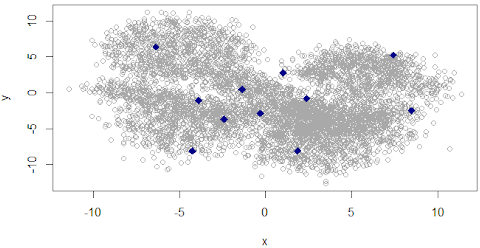
\includegraphics[width=0.8\textwidth]{images/kmeans/kmeanscloud.png}
    \end{center}
\end{frame}

\begin{frame}
\frametitle{K-means vs K-means++ Results}
    \vspace{1em}
    \begin{columns}[T] % Align columns at the top
        \column{0.4\textwidth}
        \small % Use smaller font for text
        \textbf{Standard K-means}:
            \begin{itemize}
            \item \textbf{Stats}: 5 iterations, WCSS = 22,824.
            \end{itemize}

        \vspace{1em} % Add more vertical space between the two stat blocks

        \textbf{K-means++ Initialization}:
        \vspace{-1em}
            \begin{itemize}
            \item \textbf{Stats}: 8 iterations, WCSS = 22,943.
            \end{itemize}
        
        \begin{alertblock}{Observation}
            K-means++ offered no clear advantage over standard K-means for this dataset (visually or by WCSS).
        \end{alertblock}
    

        \column{0.65\textwidth}
        \centering % Center the images
        \vspace{-2em}
        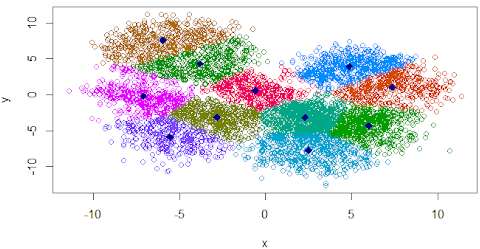
\includegraphics[width=\textwidth, height=0.55\textheight]{images/kmeans/kmeans.png} \\
        \vspace{-1em} % Space between images
        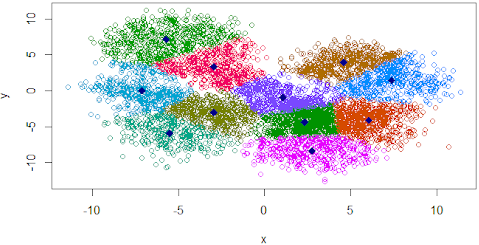
\includegraphics[width=\textwidth, height=0.55\textheight]{images/kmeans/kmeanspp.png}
    \end{columns}
    
\end{frame}



\section{Learning Commons Data}

% \begin{frame}
% \frametitle{Data Overview}
%     \begin{columns}
%         \column{0.6\textwidth}
%         \textbf{Dataset Characteristics}:
%             \begin{itemize}
%             \item Learning Commons visit records
%             \item \textbf{Train}: Fall 2016 - Spring 2017
%             \item \textbf{Test}: Fall 2017 - Spring 2018
%             \item Two prediction tasks:
%                 \begin{itemize}
%                 \item Visit Duration (in minutes)
%                 \item Occupancy at check-in
%                 \end{itemize}
%             \end{itemize}
            
%         \textbf{Key Features}:
%             \begin{itemize}
%             \item Student demographics
%             \item Academic performance metrics
%             \item Course information
%             \item Temporal visit data
%             \end{itemize}
                
%         \column{0.4\textwidth}
%         \begin{alertblock}{Prediction Tasks}
%             \begin{itemize}
%             \item Part A: Predict Duration\_In\_Min
%             \item Part B: Predict Occupancy
%             \end{itemize}
%         \end{alertblock}
%     \end{columns}
% \end{frame}

\begin{frame}
    \frametitle{Distribution Statistics}
        \begin{columns}[T]
            \column{0.4\textwidth}            
            \vspace{-0.2cm}
            \footnotesize{\textbf{Duration (minutes)}:}
            \vspace{-0.2cm}
            \begin{center}
            \footnotesize
            \begin{tabular}{>{\columncolor{bgsubrown!20}}l r}
            \toprule
            \textbf{Statistic} & \textbf{Value} \\
            \midrule
            Minimum & 6.00 \\
            1st Quartile & 44.00 \\
            Median & 68.00 \\
            Mean & 81.78 \\
            3rd Quartile & 103.00 \\
            Maximum & 822.00 \\
            \bottomrule
            \end{tabular}
            \end{center}
            
            \footnotesize{\textbf{Occupancy (students)}:}
            \vspace{-0.2cm}
            \begin{center}
            \footnotesize
            \begin{tabular}{>{\columncolor{bgsubrown!20}}l r}
            \toprule
            \textbf{Statistic} & \textbf{Value} \\
            \midrule
            Minimum & 1.00 \\
            1st Quartile & 7.00 \\
            Median & 11.00 \\
            Mean & 11.62 \\
            3rd Quartile & 15.00 \\
            Maximum & 40.00 \\
            \bottomrule
            \end{tabular}
            \end{center}
                
            \column{0.6\textwidth}
            % \footnotesize{\textbf{Distribution Plots}:}
            \vspace{0.2cm}
            
            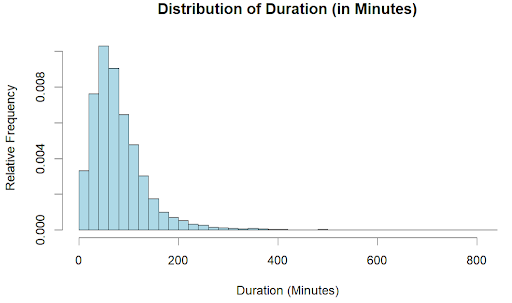
\includegraphics[width=\textwidth, height=0.46\textheight]{images/eda/dist_duration.png}
            \vspace{0.3cm}
            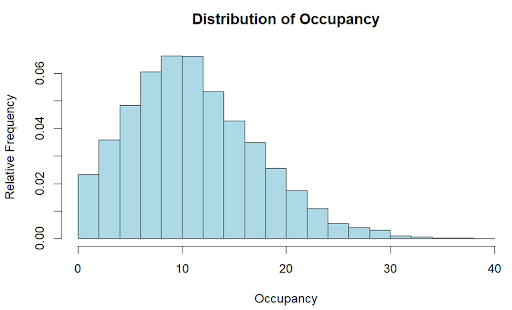
\includegraphics[width=\textwidth, height=0.41\textheight]{images/eda/dist_occupancy.png}
        \end{columns}
    
        \begin{alertblock}{Key Insight}
            Both distributions show right-skewed patterns, with some extreme values particularly in duration.
        \end{alertblock}
\end{frame}


% \section{Feature Engineering}

\begin{frame}
\frametitle{Feature Categories Overview}
    \begin{center}
    \small
    \begin{tabular}{>{\columncolor{bgsubrown!20}}l l}
    \toprule
    \textbf{Category} & \textbf{Key Features} \\
    \midrule
    Temporal & Time of day, Day of week, Week of semester \\
    \midrule
    Academic & Course level, GPA categories, Credit load \\
    \midrule
    Visit & Duration patterns, Group sizes, Visit frequency \\
    \midrule
    Course & Subject areas, Level progression, Course mix \\
    \midrule
    Student & Major groups, Class standing, Academic progress \\
    \bottomrule
    \end{tabular}

    \vspace{1em} % Add space between tables

    \hspace*{-1em} % Shift this table slightly left
    \begin{tabular}{>{\columncolor{bgsubrown!20}}m{0.3\textwidth} >{\arraybackslash}m{0.7\textwidth}}
    \toprule
    \textbf{External Source} & \textbf{Key Features} \\
    \midrule
    R library `lunar` & Moon phase data \\
    \midrule
    R library `openmeteo` & Hourly weather metrics (temperature, humidity, pressure, cloud cover, wind, radiation, precipitation, \& soil conditions) \\
    \bottomrule
    \end{tabular}
    \end{center}
\end{frame}    

\begin{frame}
\frametitle{Dropped Raw Features}
    \noindent
    \hspace{-1cm}
    % \begin{center}
    \small
    \begin{tabular}{>{\columncolor{bgsubrown!20}}l l}
    \toprule
    \textbf{Raw Feature} & \textbf{Engineered Into} \\
    \midrule
    Student\_IDs & Total\_Visits, Semester\_Visits, Avg\_Weekly\_Visits \\
    \midrule
    Class\_Standing & Class\_Standing\_Self\_Reported, Class\_Standing\_BGSU \\
    \midrule
    Major & Major\_Category, Has\_Multiple\_Majors \\
    \midrule
    Expected\_Graduation & Expected\_Graduation\_Date, Months\_Until\_Graduation \\
    \midrule
    Course\_Name & Course\_Name\_Category \\
    \midrule
    Course\_Number & Unique\_Courses, Course\_Level\_Mix \\
    \midrule
    Course\_Type & Course\_Type\_Category \\
    \midrule
    Course\_Code\_by\_Thousands & Course\_Level, Advanced\_Course\_Ratio \\
    \midrule
    \end{tabular}
    % \end{center}

    \begin{alertblock}{Feature Engineering Strategy}
        Raw features were transformed into more informative derived features, capturing higher-level patterns and relationships in the data.
    \end{alertblock}
\end{frame}

% \begin{frame}
% \frametitle{Complete Feature List (\url{~}50 Pre-Dummied)}
%     % \begin{center}
%     \noindent
%     \hspace{-1cm}
%     \footnotesize
%     \begin{tabular}{>{\columncolor{bgsubrown!20}}m{0.16\textwidth} >{\arraybackslash}m{0.93\textwidth}}
%     \toprule
%     \textbf{Category} & \textbf{Features} \\
%     \midrule
%     Student Demographics & \textbf{Student\_IDs}, Gender, \textbf{Class\_Standing}, Class\_Standing\_Self\_Reported, Class\_Standing\_BGSU, Has\_Multiple\_Majors, \textbf{Major}, Major\_Category, Degree\_Type \\
%     \midrule
%     Academic Performance & \textbf{Total\_Credit\_Hours\_Earned}, Term\_Credit\_Hours, Credit\_Load\_Category, Term\_GPA, Cumulative\_GPA, Change\_in\_GPA, GPA\_Category, GPA\_Trend \\
%     \midrule
%     Course Information & \textbf{Course\_Name}, \textbf{Course\_Number}, \textbf{Course\_Type}, Course\_Type\_Category, Course\_Level, \textbf{Course\_Code\_by\_Thousands}, Course\_Name\_Category, Course\_Level\_Mix, Advanced\_Course\_Ratio, Unique\_Courses \\
%     \midrule
%     Temporal Features & \textbf{Check\_In\_Time}, \textbf{Check\_Out\_Time}, \textbf{Check\_In\_Date}, Check\_In\_Hour, Check\_In\_Day, Check\_In\_Month, \textbf{Semester}, Semester\_Week, Check\_In\_Week, Is\_Weekend, Time\_Category \\
%     \midrule
%     Visit Metrics & \underline{\textbf{Duration\_In\_Min}}, Group\_Size, Group\_Size\_Category, Group\_Check\_In, Total\_Visits, Semester\_Visits, Week\_Volume, Avg\_Weekly\_Visits, \underline{\textbf{Occupancy}} \\
%     \midrule
%     Graduation & \textbf{Expected\_Graduation}, Expected\_Graduation\_Date, Months\_Until\_Graduation \\
%     \bottomrule
%     \end{tabular}
%     % \end{center}

%     \begin{alertblock}{Feature Set}
%         Total of 48 features used for model training, organized into logical categories.
%     \end{alertblock}
% \end{frame}


\section{Model Building}

\begin{frame}
\frametitle{Model Hyperparameter Tuning Ranges}
    \vspace{-1em} % Reduce space below title
    \begin{columns}[T] % Align columns at the top
        \hspace*{-1.5em}
        \column{0.5\textwidth}
        \centering % Center content in the column
        \textbf{Duration Task Models} \vspace{0.5em} \\ % Title for first table
        \small % Use smaller font for tables
        \begin{tabular}{>{\columncolor{bgsubrown!20}}m{0.3\textwidth} >{\arraybackslash}m{0.65\textwidth}}
        \toprule
        \textbf{Model} & \textbf{Hyperparameters} \\
        \midrule
        MARS & \textbf{num\_terms}: \([7, 15]\) \newline \textbf{prod\_degree}: 1 \\
        % \addlinespace[0.5em]
        \midrule
        Random Forest & \textbf{trees}: \([300, 325]\) \newline \textbf{min\_n}: \([15, 25]\) \newline \textbf{mtry}: \([20, 25]\) \\
        % \addlinespace[0.5em]
        \midrule
        XGBoost & \textbf{trees}: \([75, 100]\) \newline \textbf{tree\_depth}: \([15, 21]\) \newline \textbf{learn\_rate}: 0.05 \newline \textbf{min\_n}: \([10, 15]\) \newline \textbf{mtry}: \([12, 15]\) \\
        \bottomrule
        \end{tabular}
        
        \column{0.5\textwidth}
        \centering % Center content in the column
        \textbf{Occupancy Task Models} \vspace{0.5em} \\ % Title for second table
        \small % Use smaller font for tables
        \begin{tabular}{>{\columncolor{bgsubrown!20}}m{0.3\textwidth} >{\arraybackslash}m{0.65\textwidth}}
        \toprule
        \textbf{Model} & \textbf{Hyperparameters} \\
        \midrule
        MARS & \textbf{num\_terms}: \([120, 130]\) \newline \textbf{prod\_degree}: 1 \\
        % \addlinespace[0.5em]
        \midrule
        Random Forest & \textbf{trees}: \([250, 350]\) \newline \textbf{min\_n}: \([2, 3]\) \newline \textbf{mtry}: \([40, 45]\) \\
        % \addlinespace[0.5em]
        \midrule
        XGBoost & \textbf{trees}: \([350, 450]\) \newline \textbf{tree\_depth}: \([6, 8]\) \newline \textbf{learn\_rate}: 0.1 \newline \textbf{min\_n}: \([2, 3]\) \newline \textbf{mtry}: \([30, 35]\) \\
        \bottomrule
        \end{tabular}
    \end{columns}

    % \begin{alertblock}{Implementation Details}
    %     \vspace{-0.3cm}
    %     \small
    %     \begin{columns}
    %         \column{0.55\textwidth}
    %         \begin{itemize}
    %             \setlength{\itemsep}{0pt}
    %             \item \textbf{Duration}: Log-normal
    %             \item \textbf{Occupancy}: Poisson \& Weibull
    %             \item Integer rounding for occupancy
    %         \end{itemize}

    %         \column{0.45\textwidth}
    %         \begin{itemize}
    %             \setlength{\itemsep}{0pt}
    %             \item Grid search optimization
    %             \item Feature selection
    %             \item Cross-validation
    %         \end{itemize}            
    %     \end{columns}
    % \end{alertblock}
    
\end{frame}

\begin{frame}
\frametitle{Deep Learning Hyperparameters}
    \vspace{-1em} % Reduce space below title
    \begin{columns}[T] % Align columns at the top
        \hspace*{-1.5em}
        \column{0.5\textwidth}
        \centering % Center content in the column
        \textbf{Duration Task Models} \vspace{0.5em} \\ % Title for first table
        \footnotesize  % Use smaller font for tables
        \begin{tabular}{>{\columncolor{bgsubrown!20}}m{0.15\textwidth} >{\arraybackslash}m{0.8\textwidth}}
        \toprule
        \textbf{Model} & \textbf{Hyperparameters} \\
        \midrule
        GRU & \textbf{lr}: \([10^{-3}, 5 \times 10^{-3}]\) \newline \textbf{batch\_size}: \(\{64, 128\}\) \newline \textbf{gru\_dim}: \(\{128, 256, 512\}\) \newline \textbf{num\_layers}: \(\{1, 2\}\) \newline \textbf{gru\_expansion}: \([0.5, 1.4]\) \newline \textbf{dropout\_rate}: \([0.25, 0.42]\) \newline \textbf{weight\_decay}: \([10^{-6}, 10^{-5}]\) \newline \textbf{activation\_fn}: relu \\
        % \addlinespace[0.5em]
        \midrule
        Trans-former & \textbf{lr}: \([10^{-3}, 7 \times 10^{-3}]\) \newline \textbf{batch\_size}: 64 \newline \textbf{d\_model}: 128 \newline \textbf{nhead}: \(\{4, 8\}\) \newline \textbf{nlayers}: \(\{2, 3\}\) \newline \textbf{d\_hid}: 128 \newline \textbf{dropout}: \([0.05, 0.20]\) \newline \textbf{weight\_decay}: \([10^{-6}, 10^{-4}]\) \\
        \bottomrule
        \end{tabular}
        
        \column{0.5\textwidth}
        \centering % Center content in the column
        \textbf{Occupancy Task Models} \vspace{0.5em} \\ % Title for second table
        \footnotesize  % Use smaller font for tables
        \begin{tabular}{>{\columncolor{bgsubrown!20}}m{0.15\textwidth} >{\arraybackslash}m{0.8\textwidth}}
        \toprule
        \textbf{Model} & \textbf{Hyperparameters} \\
        \midrule
        GRU & \textbf{lr}: \([1.2 \times 10^{-3}, 5 \times 10^{-3}]\) \newline \textbf{batch\_size}: \(\{64, 128\}\) \newline \textbf{gru\_dim}: 512 \newline \textbf{num\_layers}: 2 \newline \textbf{gru\_expansion}: \([0.6, 1.4]\) \newline \textbf{dropout\_rate}: \([0.25, 0.42]\) \newline \textbf{weight\_decay}: \([10^{-6}, 5 \times 10^{-6}]\) \newline \textbf{activation\_fn}: relu \\
        % \addlinespace[0.5em]
        \midrule
        Trans-former & \textbf{lr}: \([8 \times 10^{-4}, 1.5 \times 10^{-3}]\) \newline \textbf{batch\_size}: \(\{64, 128\}\) \newline \textbf{d\_model}: \(\{64, 128, 256\}\) \newline \textbf{nhead}: \(\{4, 8\}\) \newline \textbf{nlayers}: \(\{2, 3\}\) \newline \textbf{d\_hid}: 128 \newline \textbf{dropout}: \([0.05, 0.20]\) \newline \textbf{weight\_decay}: \([10^{-6}, 10^{-5}]\) \\
        \bottomrule
        \end{tabular}

    \end{columns}
\end{frame}

\begin{frame}
\frametitle{Preprocessing Pipeline Details}
    % Removed KFold text, using columns layout
    \begin{columns}[T] % Use columns for layout
        \column{0.6\textwidth} % Column for Recipe steps
        \begin{block}{R `recipes` Pipeline Steps}
        \small % Smaller font for the list
        \begin{enumerate}
            \item Define roles (outcome, predictors)
            \item Remove specified ID/date/unwanted columns
            \item Convert \texttt{Check\_In\_Time} to minutes past midnight
            \item Impute missing numerics (mean)
            \item Handle novel factor levels
            \item Create dummy variables (drop first)
            \item Remove zero-variance predictors
            \item Normalize numeric predictors
        \end{enumerate}
        \end{block}
        
        \column{0.4\textwidth} % Column for Explanation
        \begin{alertblock}{Step 5: Handling Novel Factor Levels}
        \footnotesize % Use footnotesize for the detailed explanation
        Prepares for unseen categories in new data:
            \begin{itemize}
                \item Adds a special "novel" level to factors.
                \item Replaces unknown categories with "novel" instead of causing errors.
                \item Ensures robust predictions, especially before dummy encoding.
            \end{itemize}
        \end{alertblock}

    \end{columns}
\end{frame}

\section{Evaluation}

\begin{frame}
\frametitle{Top Model Performance (Holdout Set)}
    \begin{columns}[T] % Use columns for layout
        \column{0.5\textwidth}
        \centering % Center content in the column
        \textbf{Duration Task} \vspace{0.5em} \\ % Title for first table
        %\small
        \begin{tabular}{>{\columncolor{bgsubrown!20}}l r r}
        \toprule
        \textbf{Model} & \textbf{RMSE} & \textbf{R²} \\
        \midrule
        XGBoost & 59.9 & 0.099 \\
        \midrule
        Random Forest & 60.1 & 0.090 \\
        \midrule
        Transformer & 61.3 & 0.010 \\
        \midrule
        MARS & 61.6 & 0.045 \\
        \midrule
        GRU & 63.8 & 0.041 \\
        \bottomrule
        \end{tabular}
        
        \column{0.5\textwidth}
        \centering % Center content in the column
        \textbf{Occupancy Task} \vspace{0.5em} \\ % Title for second table
        %\small
        \begin{tabular}{>{\columncolor{bgsubrown!20}}l r r}
        \toprule
        \textbf{Model} & \textbf{RMSE} & \textbf{R²} \\
        \midrule
        XGBoost & 1.83 & 0.911 \\
        \midrule
        Random Forest & 1.93 & 0.902 \\
        \midrule
        GRU & 3.16 & 0.738 \\
        \midrule
        Transformer & 3.26 & 0.706 \\
        \midrule
        MARS & 3.78 & 0.617 \\
        \bottomrule
        \end{tabular}

    \end{columns}
    
    \vspace{1em} % Add space before alert block
    \begin{alertblock}{Key Performance Observations}
        \small % Use smaller font for alert block
        Based on holdout set metrics:
        \begin{itemize}
            \setlength{\itemsep}{0pt}
            \setlength{\parsep}{0pt}
            \setlength{\topsep}{0pt}
            \item \textbf{Duration Task:} XGBoost achieved the lowest RMSE (59.9) and highest R² (0.099).
            \item \textbf{Occupancy Task:} XGBoost also performed best, with the lowest RMSE (1.83) and highest R² (0.911).
        \end{itemize}
    \end{alertblock}
\end{frame}

\begin{frame}
    \frametitle{Best Model Configurations}
        \begin{columns}[T]
            \column{0.48\textwidth}
            \textbf{Duration Prediction}:
            \vspace{-0.5cm}
            \begin{center}
            \small
            \begin{tabular}{>{\columncolor{bgsubrown!20}}l l}
            \toprule
            \textbf{Component} & \textbf{Value} \\
            \midrule
            Model & PenalizedSplines \\
            Pipeline & vanilla \\
            CV Method & kfold \\
            RMSE & 59.47 \\
            R² & 0.059 \\
            \midrule
            Ridge $\alpha$ & 14.38 \\
            Spline degree & 3 \\
            Spline knots & 15 \\
            Scaler & RobustScaler \\
            \bottomrule
            \end{tabular}
            \end{center}
                
            \column{0.48\textwidth}
            \textbf{Occupancy Prediction}:
            \vspace{-0.5cm}
            \begin{center}
            \small
            \begin{tabular}{>{\columncolor{bgsubrown!20}}l l}
            \toprule
            \textbf{Component} & \textbf{Value} \\
            \midrule
            Model & PenalizedSplines \\
            Pipeline & vanilla \\
            CV Method & rolling \\
            RMSE & 3.64 \\
            R² & 0.303 \\
            \midrule
            Ridge $\alpha$ & 29.76 \\
            Spline degree & 3 \\
            Spline knots & 15 \\
            Scaler & RobustScaler \\
            \bottomrule
            \end{tabular}
            \end{center}
        \end{columns}
    
        \begin{alertblock}{Key Insight}
            Both tasks achieved best results with PenalizedSplines and vanilla features, though with different CV methods \& regularization.
        \end{alertblock}
    \end{frame}
    
\begin{frame}
\frametitle{Duration: Best Model Diagnostics}
    \begin{center}
        \noindent\centering
        \vspace{-0.7cm}
        % 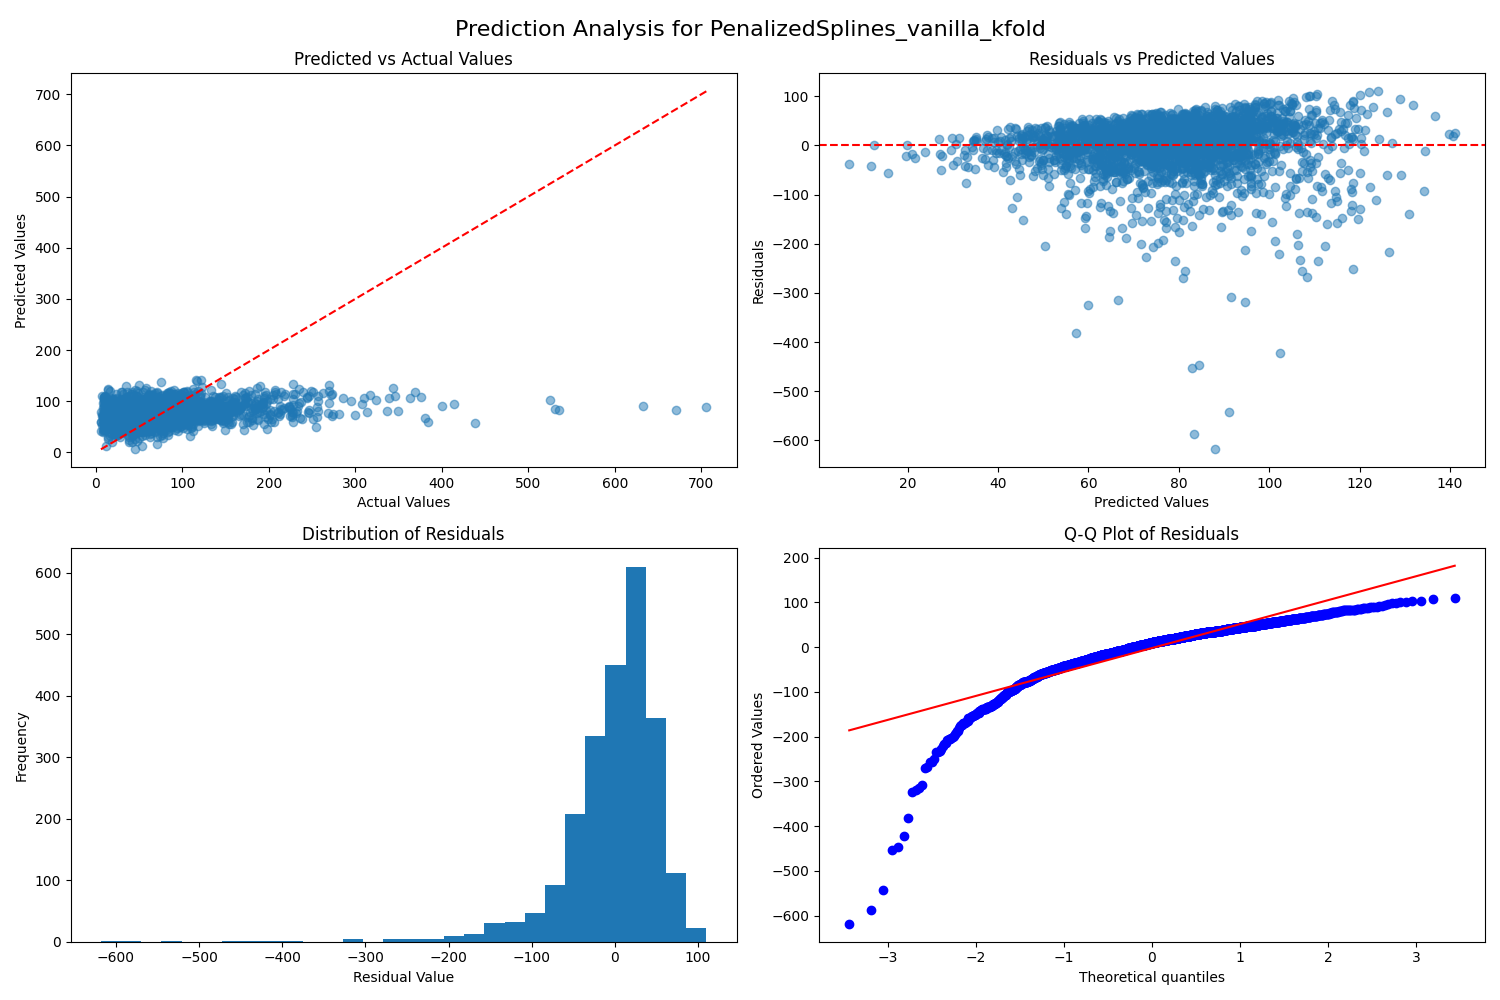
\includegraphics[width=1.0\textwidth, height=0.95\textheight,
        %     % keepaspectratio,    % Maintains aspect ratio
        %     interpolate=false,  % Prevents blurry interpolation
        %     draft=false]{images/evaluation/Duration_PenalizedSplines_vanilla_kfold.jpg}
    \end{center}
\end{frame}

\begin{frame}
\frametitle{Occupancy: Best Model Diagnostics}
    \begin{center}
        \noindent\centering
        \vspace{-0.7cm}
        % 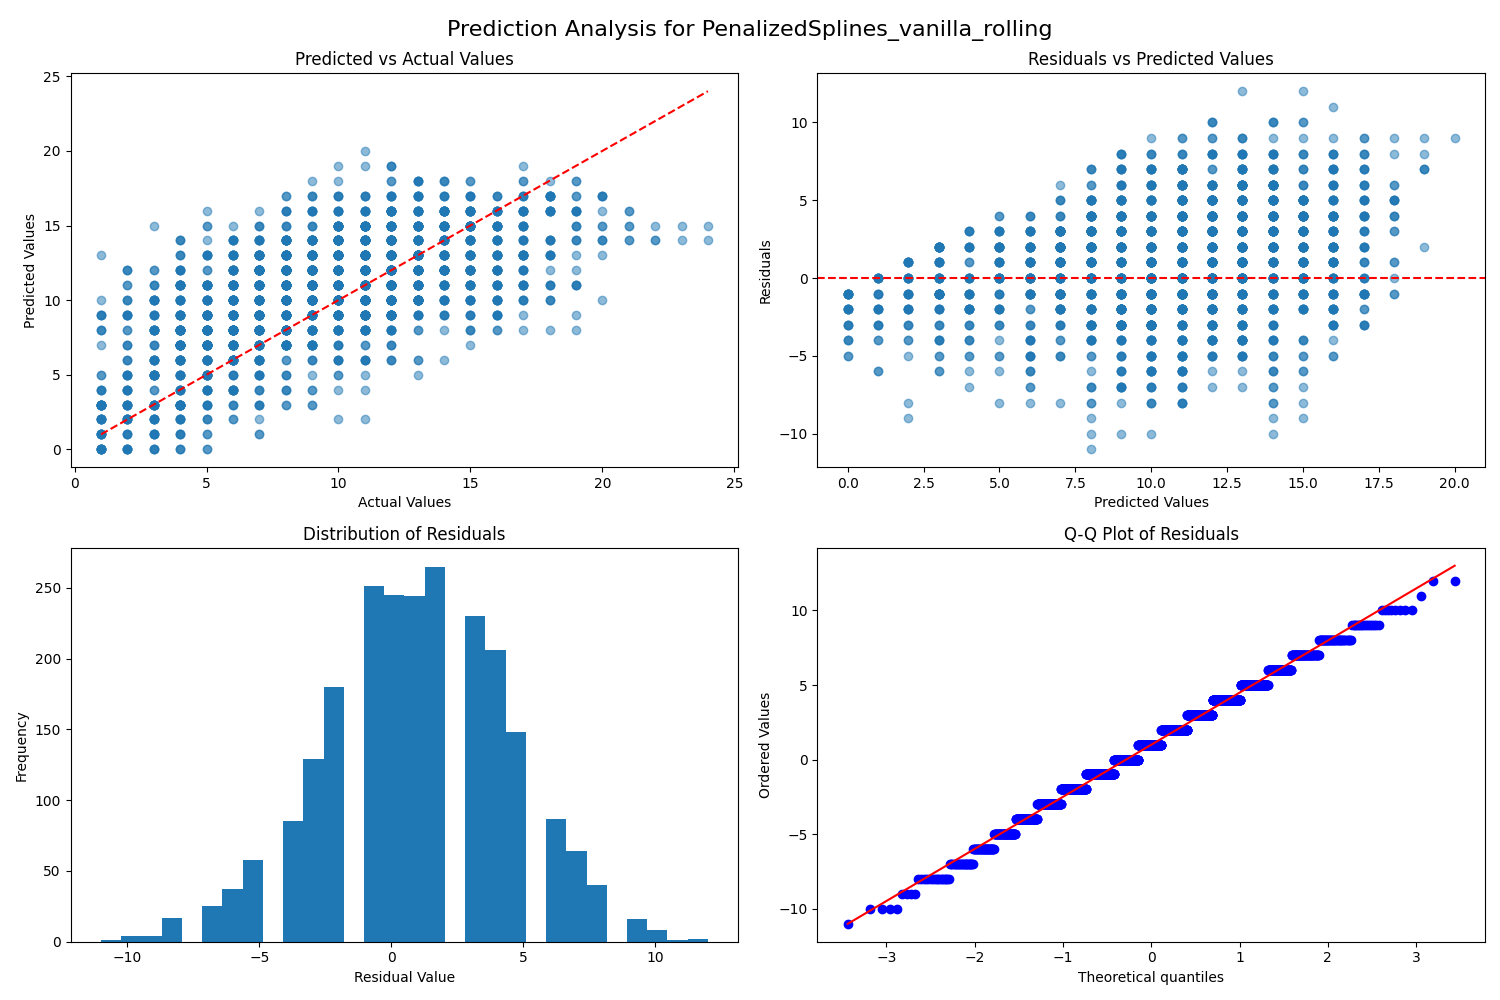
\includegraphics[width=1.0\textwidth, height=0.95\textheight,
        %     % keepaspectratio,    % Maintains aspect ratio
        %     interpolate=false,  % Prevents blurry interpolation
        %     draft=false]{images/evaluation/Occupancy_PenalizedSplines_vanilla_rolling.jpg}
    \end{center}
\end{frame}

\begin{frame}
\frametitle{Sanity Check}
    \vspace{-0.35cm}
    \begin{center}
        % Top image
        % 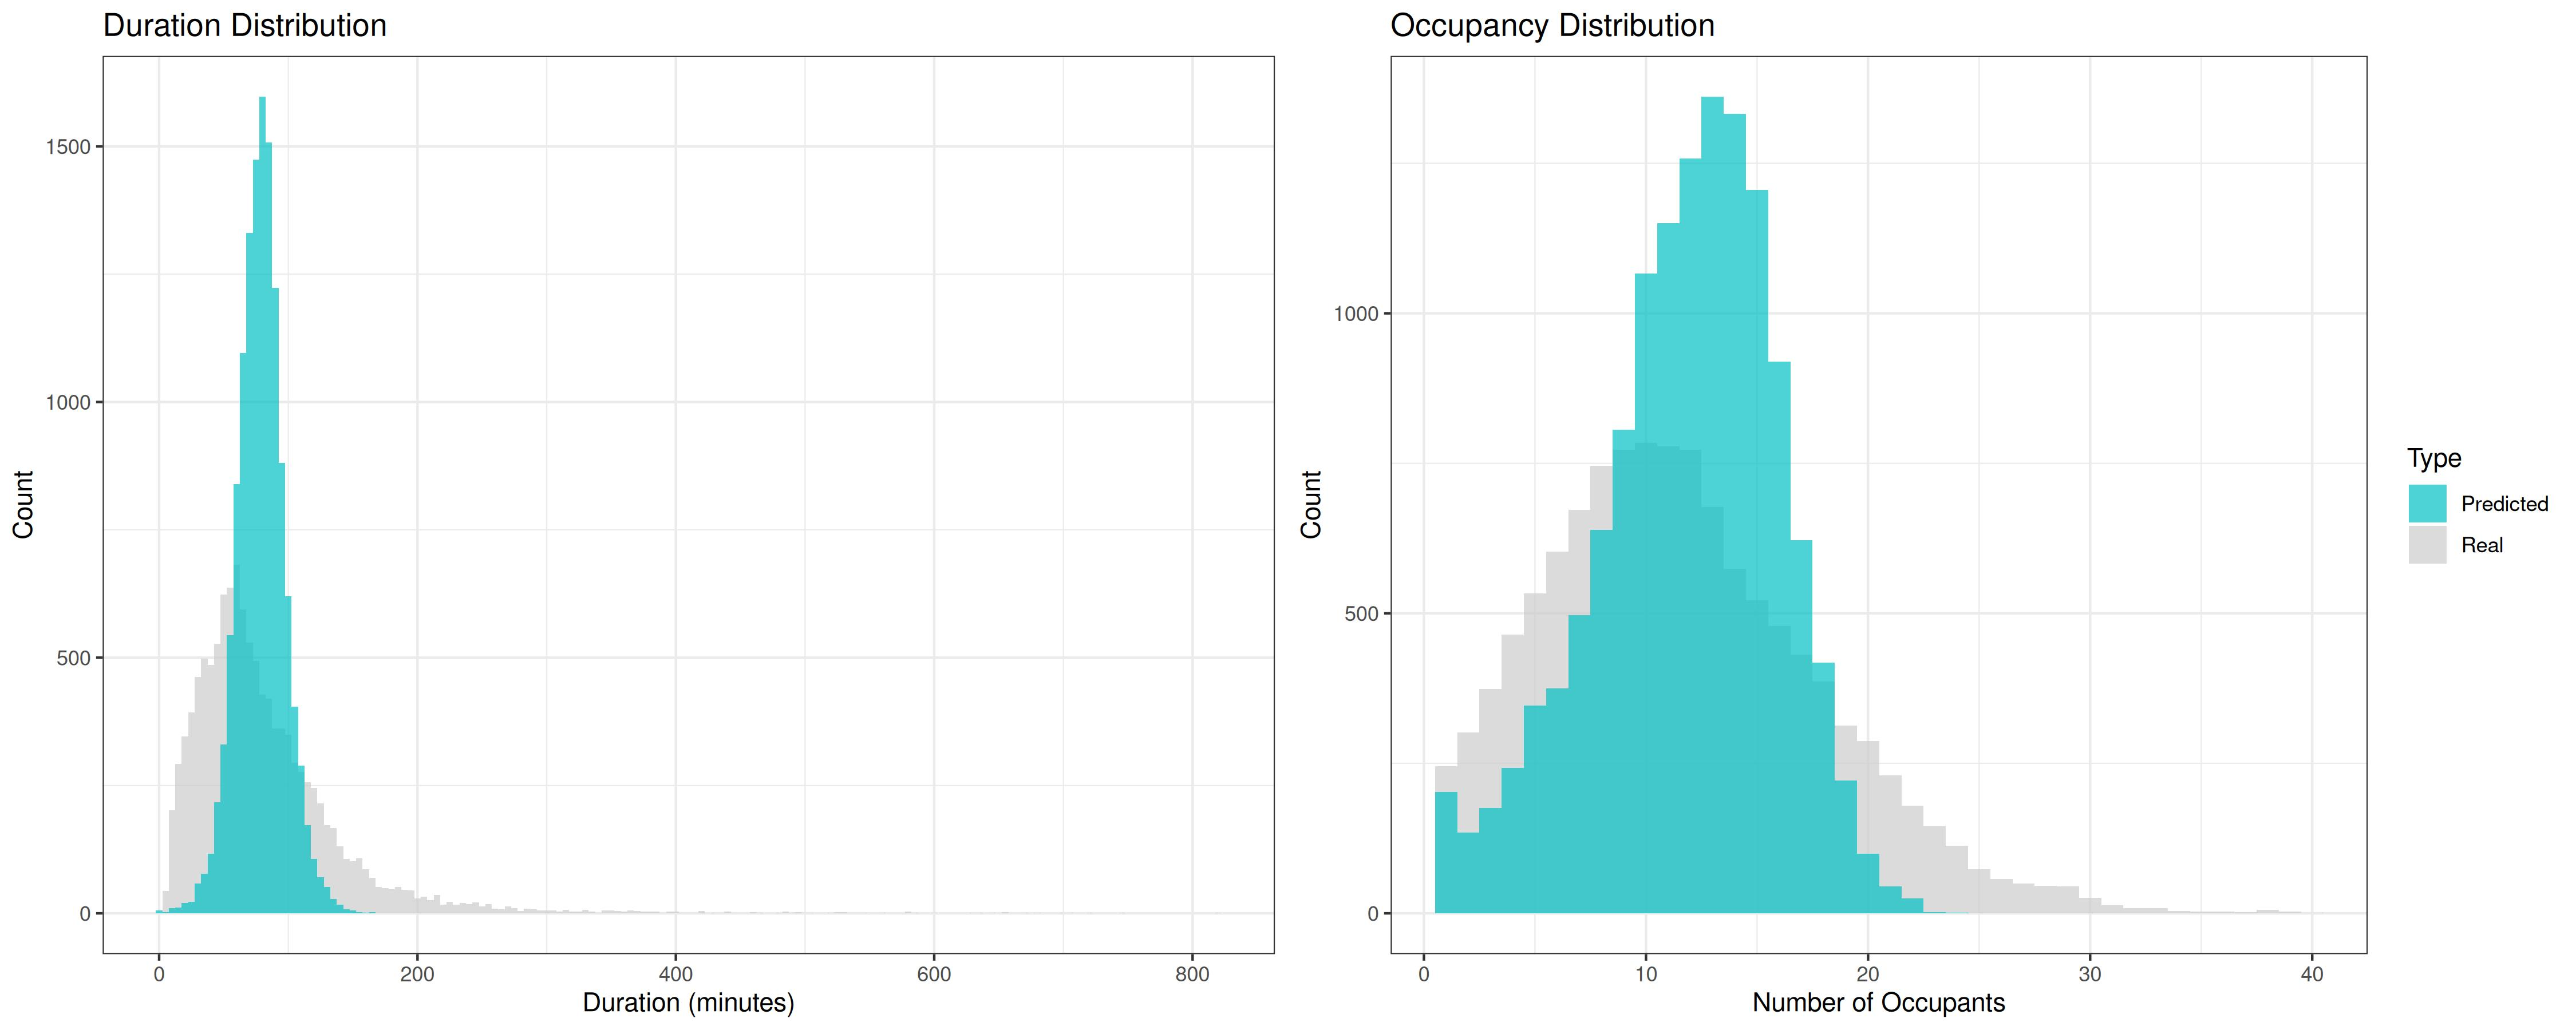
\includegraphics[width=1.0\textwidth, height=0.49\textheight]{images/evaluation/distribution_comparisons.jpg}
        
        \vspace{0.1cm} % Add some vertical spacing between images
        
        % Bottom image
        % 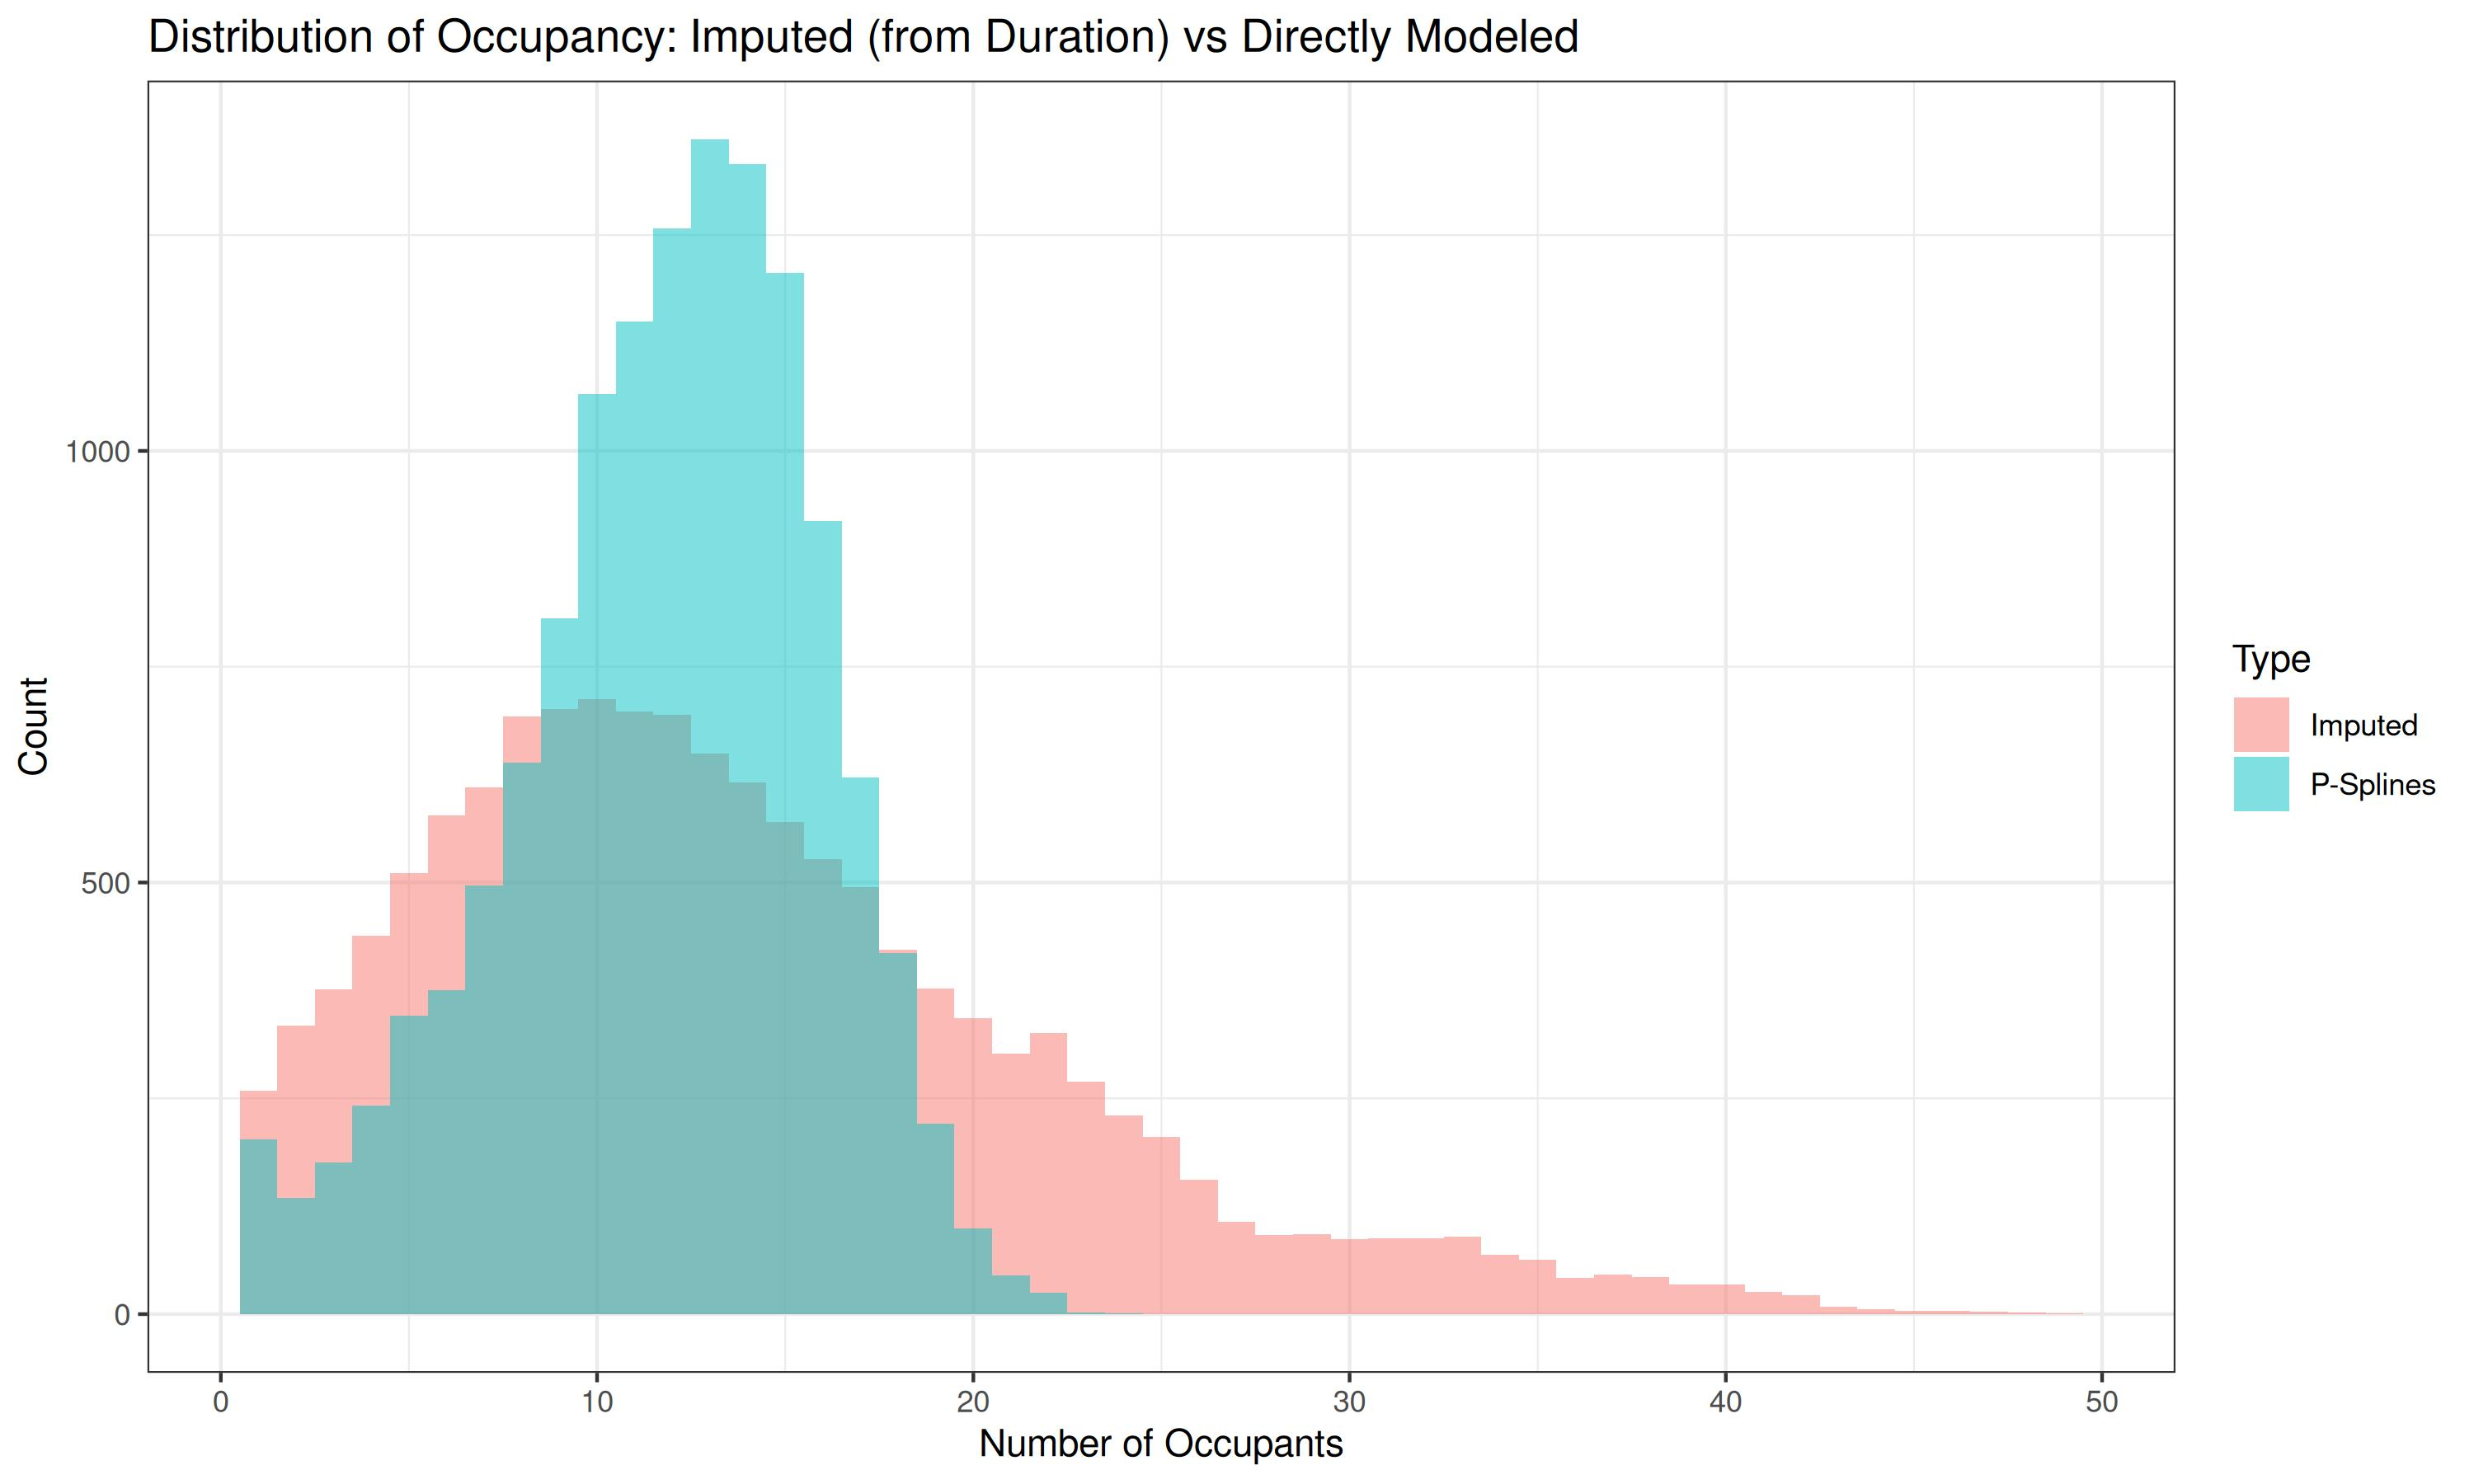
\includegraphics[width=1.0\textwidth, height=0.45\textheight]{images/evaluation/occupancy_comparison_histogram.jpg}

    \end{center}
\end{frame}

\section{Conclusion}

\begin{frame}
\frametitle{Key Findings}
    \begin{columns}
        \column{0.55\textwidth}
        \textbf{Main Results}:
            \begin{itemize}
                \item \textbf{PenalizedSplines} with \textit{vanilla} features performed best
                \item \textbf{Occupancy} prediction shows promise (R² = 0.303)
                \item \textbf{Duration} prediction remains challenging (R² = 0.059)
            \end{itemize}
                            
        \column{0.5\textwidth}
        \textbf{Future Directions}:
            \begin{itemize}
            \item Incorporate \textit{weather} data
            \item Explore \textit{non-linear} relationships further
            \item Investigate \textit{time series} approaches
            \end{itemize}
    \end{columns}

    \vspace{0.5cm}
    \begin{alertblock}{Impact}
        While duration prediction remains difficult, our occupancy model shows strong potential for a victory \textbf{\#CautiousOptimism}
    \end{alertblock}
\end{frame}

\appendix
\begin{frame}[plain]
\begin{center}
    \vspace{-0.5cm}
    \begin{tikzpicture}[remember picture,overlay]
        % Decorative border
        \draw[line width=2pt, bgsubrown] 
            ([shift={(0.5cm,0.5cm)}]current page.south west) 
            rectangle 
            ([shift={(-0.5cm,-0.5cm)}]current page.north east);
        
        \draw[line width=1pt, bgsuorange] 
            ([shift={(0.7cm,0.7cm)}]current page.south west) 
            rectangle 
            ([shift={(-0.7cm,-0.7cm)}]current page.north east);
        
        % Ornamental corners
        \foreach \corner in {north east, north west, south east, south west} {
            \draw[bgsubrown, line width=1.5pt] 
                ([shift={(0.5cm,0.5cm)}]current page.\corner) 
                -- ++(45:0.3cm) -- ++(135:0.3cm);
        }
    \end{tikzpicture}

    \vspace{1cm}
    {\Huge\calligra Thank You}
    \vspace{0.8cm}
    
    \begin{center}
        \begin{tabular}{c}
            {\large\calligra For Your Attention} \\[0.5cm]
            \hline \\[0.1cm]
            {\small Questions \& Discussion Welcome}
        \end{tabular}
    \end{center}
\end{center}
\end{frame}

\end{document} 